\section{DINÁMICA ROTACIONAL}
\subsection{Análisis de Torque}
\begin{frame}{DINÁMICA ROTACIONAL}
\framesubtitle{Análisis de Torque}
	En el golf podemos evidenciar rotación en cuatro partes:
    \begin{itemize}
    \item Rotación bola de golf.
    \item Rotación palo y brazos.
    \item Rotación de las caderas.
    \item Rotación de las piernas.
    \end{itemize}

	\begin{figure}[H]
      \centering
      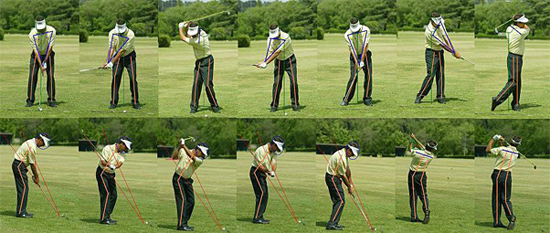
\includegraphics[scale = 0.375]{Swing.jpg}
      \caption{Movimiento durante un swing\footnotemark{}.}
    \end{figure}
     \vspace{-2cm}\footnotetext{\bibentry{swing1}.}
\end{frame}

%%%%%%%%%%%%%%%%%%%%%%%%%%%%
\subsection{Torque palo de golf}
\begin{frame}{DINÁMICA ROTACIONAL}
\framesubtitle{Torque palo de golf}
Para analizar dicho torque, hay que tener en cuenta:\begin{itemize}
\item Eje de rotación
\item El sistema
\end{itemize}
\begin{figure}[H]
      \centering
      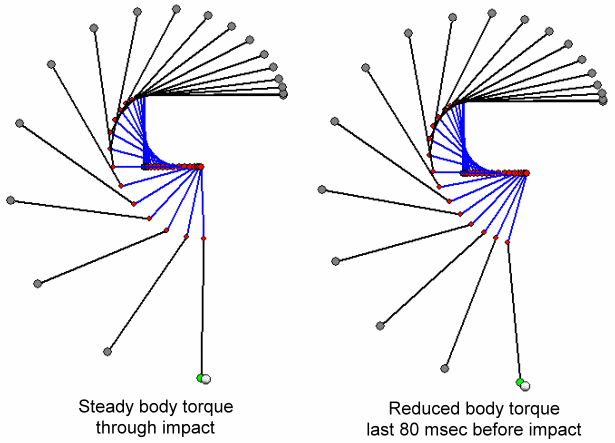
\includegraphics[scale = 0.275]{Movement_body.jpg}
      \caption{Sistema rotacional para el torque.}
\end{figure}
\end{frame}

%%%%%%%%%%%%%%%%%%%%%%%%%%%%%
\begin{frame}{DINÁMICA ROTACIONAL}
\framesubtitle{Torque palo de golf}
Con todo lo dicho, podriámos considerar el sistema como un péndulo doble.
\begin{figure}[H]
      \centering
      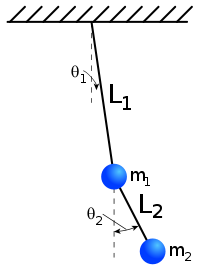
\includegraphics[scale = 0.3]{Double_Pendulum.png}
      \caption{Sistema de péndulo doble.}
\end{figure}
\begin{equation}
\alpha =\frac { 2\sin { ({ \theta  }_{ 1 }-\theta )\left( { { c }_{ 1 } }{ \omega  }_{ 1 }^{ 2 }+c_{ 2 }\cos { { \theta  }_{ 1 } } +{ c }_{ 3 }{ \omega  }^{ 2 }\cos { \left( { { \theta  }_{ 1 }-\theta  } \right)  }  \right)  }  }{ { c }_{ 4 }-{ c }_{ 5 }\cos { (2\left( { \theta  }_{ 1 }-\theta  \right) ) }  } 
\end{equation}
\end{frame}
%%%%%%%%%%%%%%%%%%%%%%%%%%%%%%%%%%%%%%%%%%%%%%%%%
\subsection{Efecto Magnus}
\begin{frame}{DINÁMICA ROTACIONAL}
\framesubtitle{Efecto Magnus}
\url{https://www.youtube.com/watch?v=2OSrvzNW9FE}\quad(0:00 - 1:24).
\begin{figure}[H]
      \centering
      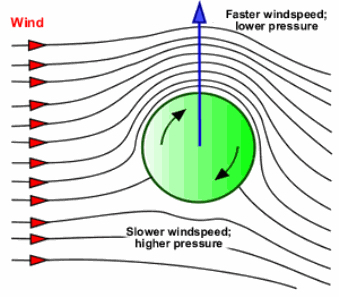
\includegraphics[scale = 0.3]{Magnus.jpg}
      \caption{Efecto magnus en un cuerpo esférico.}
\end{figure}
\begin{equation}
\frac { 1 }{ 2 } \rho { v }^{ 2 }+\rho gh+P=Cte
\end{equation}
\end{frame}
%%%%%%%%%%%%%%%%%%%%%%%%%%%%%%%%%%%%%%%%%%%%%%
\begin{frame}{DINÁMICA ROTACIONAL}
\framesubtitle{Efecto Magnus}
Para una esfera, la fuerza que hace este efecto sería apróximadamente:
\begin{equation}
\vec { F } \approx \left( { \pi  }^{ 2 }{ r }^{ 3 }\rho  \right) \vec { \omega  } \times \vec { v } 
\end{equation}
\begin{figure}[H]
      \centering
      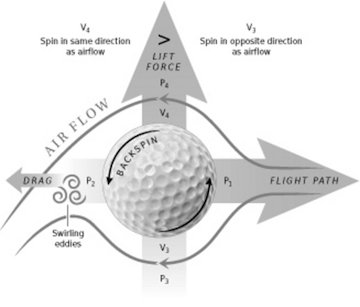
\includegraphics[scale = 0.385]{Golf_Magnus.jpg}
      \caption{Efecto magnus en un cuerpo esférico.}
\end{figure}
\end{frame}
%%%%%%%%%%%%%%%%%%%%%%%%%%%%%%%%%%%%%%%%%%%%%
\subsection{Torque bola de golf}
\begin{frame}{DINÁMICA ROTACIONAL}
\framesubtitle{Torque bola de golf}
Hay tres tipos de rotaciones con efectos positivos y una con efectos negativos.
\begin{itemize}
	\item Hook
	\item Slice
	\item Backspin
	\item \textbf{Overspin}
\end{itemize}
\end{frame}